\documentclass[twoside]{report}

% Use so that < and > get formatted correctly when printed in text
%\usepackage[T1]{fontenc}
\usepackage{acronym}
\usepackage{amsmath}
%\usepackage{array}
\usepackage[blocks]{authblk}
%\usepackage{booktabs}
%\usepackage[toc]{appendix}
%\usepackage{breqn}
\usepackage[justification=justified,singlelinecheck=off,bf]{caption}
\usepackage{chngcntr}
\usepackage{changepage}
\usepackage[usenames,dvipsnames]{color}
\usepackage{enumerate}
\usepackage{enumitem}
\usepackage{fancyhdr}
%\usepackage[Glenn]{fncychap}
\usepackage{fancybox}
\usepackage{fancyvrb}
\usepackage{float}
%\usepackage{framed}
%\usepackage{fullpage}
%\usepackage{gensymb}
\usepackage[top=1.0in,bottom=1.0in,inner=1.0in,outer=1.0in]{geometry}
\usepackage{graphicx}
\usepackage{lastpage}
%\usepackage{listing}
%\usepackage{lscape}
%\usepackage{makecell}
%\usepackage{multirow}
%\usepackage{pdflscape}
\usepackage{units}
\usepackage{newfloat}
\usepackage{wrapfig}
%\usepackage{nicefrac}
%\usepackage{multicol}
%\usepackage{xr-hyper}
\usepackage{hyperref}
\usepackage{tabularx}
\usepackage{siunitx}
\usepackage{textcomp}
\usepackage[pages=some]{background}
\usepackage{longtable}
\usepackage{booktabs}
\usepackage{titlesec}

\newcommand{\CASLMilestoneNumber}{CASL-U-2019-1878-002}
\title{VERAIO Software Management Plan}
\newcommand{\subtitle}{}
\newcommand{\shortTitle}{VERAIO Software Management Plan}
\newcommand{\psm}{Erik Walker, VERAIO Product Software Manager}
\newcommand{\reviewer}{Aaron Graham, Independent Reviewer}
\newcommand{\techlead}{Benjamin Collins, Program Technical Leader}
\newcommand{\veraqm}{Tristan Grover, VERA Software Quality Coordinator}
\author[1]{Scott Palmtag}
\author[2]{Erik Walker}
\affil[1]{North Carolina State University}
\affil[2]{Oak Ridge National Laboratory}

% Special thanks to authors of CTF and MPACT SMP documents!
%    Bob Salko
%    Thomas Downar
%    Brendan Kochunas
%    Shane Stimpson
%    Benjamin Collins

\newcommand{\publicationDate}{3/3/2021}

%customize hyperref
%uncomment to underline the hyperlinks in the document
\hypersetup{
        colorlinks,
%	colorlinks=false,
%	pdfborderstyle={/S/U/W 1},
%	pdfborder=0 0 1,
	linkcolor=black,
	citecolor=black,
	}


% Make custom blue to match word blue
\definecolor{DocNameBlue}{RGB}{154,189,251}
% CASL blue
\definecolor{CASLBlue}{RGB}{0,132,246}
\definecolor{TitleBlue}{RGB}{37,65,96}


% All the other pages style
\renewcommand{\headrulewidth}{0pt}
\fancyhead{}
\fancyfoot{}
\fancyhead[LO,RE]{
\includegraphics[width=1.5in]{template/CASL_logo.png}}
\fancyhead[RO,LE]{\color{CASLBlue}\shortTitle}
\fancyfoot[LE,RO]{\textcolor{CASLBlue}{C}onsortium for \textcolor{CASLBlue}{A}dvanced \textcolor{CASLBlue}{S}imulation of \textcolor{CASLBlue}{L}WRs}
\fancyfoot[RE,LO]{\CASLMilestoneNumber}
\fancyfoot[CO,CE]{\thepage}

\fancypagestyle{plain}
{
\fancyhead[LO,RE]{
\includegraphics[width=1.5in]{template/CASL_logo.png}}
\fancyhead[RO,LE]{\color{CASLBlue}\shortTitle}
\fancyfoot[LE,RO]{\textcolor{CASLBlue}{C}onsortium for \textcolor{CASLBlue}{A}dvanced \textcolor{CASLBlue}{S}imulation of \textcolor{CASLBlue}{L}WRs}
\fancyfoot[RE,LO]{\CASLMilestoneNumber}
\fancyfoot[CO,CE]{\thepage}
}

% The title page style
\fancypagestyle{firststyle}
{
   \fancyhead[L]{}
   \fancyhead[R]{\CASLMilestoneNumber}
   \fancyfoot[]{}
}


\backgroundsetup{
scale=1,
color=black,
opacity=1.0,
angle=0,
contents={%
  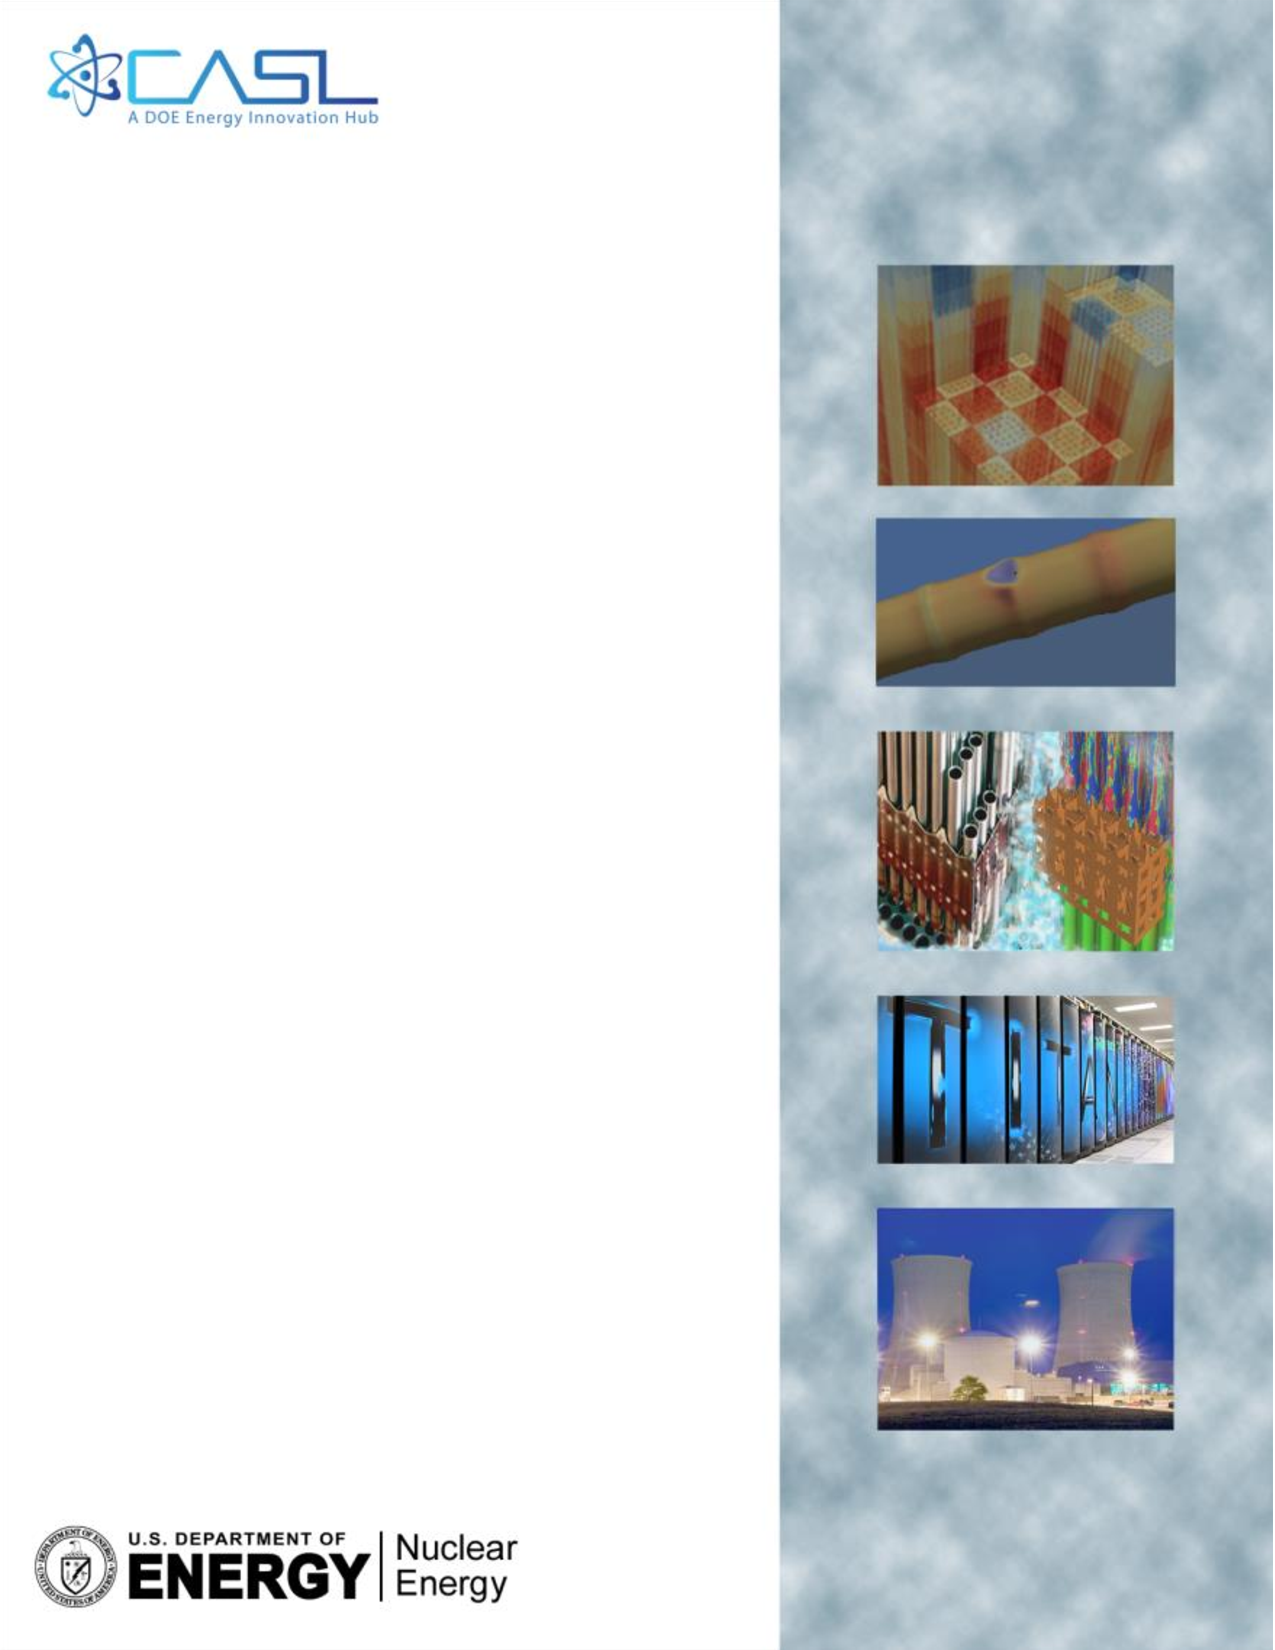
\includegraphics[width=\paperwidth,height=\paperheight]{template/casl_background.pdf}
  }%
}

% Define command to surround text in angle brackets
\newcommand{\brackets}[1]{\textlangle{}#1\textrangle{}}

% For formatting code
\newcommand{\codeblock}[1]{\texttt{#1}}


% define documents that are referenced often
\newcommand{\VERAReq}{{\it VERA-QA-006, VERA Requirements and Design Process}}


%increase space after captions
\setlength{\belowcaptionskip}{2pt}

% No indenting at start of paragraph
\setlength{\parindent}{0pt}

%increase space between paragraphs
\parskip 1em

\titleformat{\chapter}{\Huge\bfseries}{\thechapter. }{0pt}{\Huge\bfseries}

% set the section numbering depth and TOC depth
\setcounter{secnumdepth}{3}
\setcounter{tocdepth}{3}

% Use continuous counting scheme for floats
\counterwithout{table}{chapter}

\let\DeclareUSUnit\DeclareSIUnit
\let\US\SI
\DeclareUSUnit\F{F}
\DeclareUSUnit\ft{ft}

% Set list spacing to zero
%\setitemize{itemsep=0em}

\begin{document}

%clear the header/footer until TOC
\pagenumbering{roman}

\begin{titlepage}

   \BgThispage
   \thispagestyle{firststyle}
   
   \vspace*{\fill}
   
   \begin{minipage}[l][][c]{0.6\textwidth}
   \begin{flushleft}
   \makeatletter
   {\huge\color{TitleBlue}\bf Consortium for Advanced \\\vspace{0.3cm} Simulation of LWRs}\\
   \vspace{3cm}
   {\huge\fontfamily{phv}\selectfont\color{TitleBlue}\bf
   % Title of the document
   \@title\par
   }
   {\Large\fontfamily{phv}\selectfont\color{DocNameBlue}\bf
   \subtitle\par
   }
   \vspace*{30pt}
   % Authors
   {\Large\bf\setlength{\parskip}{10pt}
   \@author
   
   }
   \vspace*{30pt}
   {\huge\bf
   \publicationDate
   }
   \makeatother
   
   
   \end{flushleft}
   \end{minipage}
   
   \vspace*{\fill}
   
\begin{minipage}{0.6\textwidth}
   
\includegraphics[width=\textwidth]{template/verabanner.png}
\end{minipage}

\vspace{1cm}

   
   \end{titlepage}

   \pagestyle{fancy}

   \vspace*{\fill}

   \captionsetup{justification=centering}
   \begin{table}[H]
   \centering
   \caption*{\Large\bfseries{Revision Log}}
   \begin{tabular}{rrrr}
   \toprule
   \textbf{Revision} & \textbf{Date} & \textbf{Affected Pages} & \textbf{Revision Description} \\
   \midrule
   0 & \publicationDate & All & Initial Release \\
   & & & \\
   & & & \\
   & & & \\
   & & & \\
   & & & \\
   & & & \\
   \bottomrule
   \end{tabular}
   \end{table}
   
   \vspace*{\fill}
   
   
   \begin{table}[H]
   \caption*{\Large\bfseries{Document pages that are:}}
   \centering
   \begin{tabular}{ll}
   Export Controlled: & None \\
   IP/Proprietary/NDA Controlled: & None \\
   Sensitive Controlled: & None \\
   Unlimited: & All \\
   \end{tabular}
   \end{table}
   
   \vspace*{\fill}
   
   This document was prepared as an account of work sponsored by an agency of the United States Government. Neither the United States Government nor any agency thereof, nor any of their employees, makes any warranty, express or implied, or assumes any legal liability or responsibility for the accuracy, completeness, or usefulness of any information, apparatus, product, or process disclosed, or represents that its use would not infringe privately owned rights. Reference herein to any specific commercial product, process, or service by trade name, trademark, manufacturer, or otherwise, does not necessarily constitute or imply its endorsement, recommendation, or favoring by the United States Government or any agency thereof. The views and opinions of authors expressed herein do not necessarily state or reflect those of the United States Government or any agency thereof.

   \captionsetup{justification=justified}
   
   \vspace*{\fill}
\clearpage 

\makeatletter
\begin{center}
{\huge\bf\@title\par}
\end{center}

\vspace{2cm}

{\Large\bf Approvals:}

\vspace{2cm}

\begin{tabular}{ll}
\makebox[3.5in]{\hrulefill} & \makebox[2.0in]{\hrulefill}\\
{\bf\psm} & {\bf Date}\\[3cm]
\makebox[3.5in]{\hrulefill} & \makebox[2.0in]{\hrulefill}\\
{\bf\reviewer} & {\bf Date}\\[3cm]
\makebox[3.5in]{\hrulefill} & \makebox[2.0in]{\hrulefill}\\
{\bf\techlead} & {\bf Date}\\[3cm]
\makebox[3.5in]{\hrulefill} & \makebox[2.0in]{\hrulefill}\\
{\bf\veraqm} & {\bf Date}\\[3cm]
\end{tabular}

\makeatother

\clearpage

% no abstract in users' manual
%\begin{center}
  {\large \bfseries \noindent Abstract}
\end{center}

Add Abstract here  (not part of SMP)


\chapter*{Acronyms}
\begin{acronym}
\acro{casl}[CASL]{Consortium for the Advanced Simulation of Light Water Reactors}
\acro{gui}[GUI]{graphical user interface}
\acro{hpc}[HPC]{high performance computing}
\acro{ornl}[ORNL]{Oak Ridge National Laboratory}
\acro{phi}[PHI]{physics integration}
\acro{psm}[PSM]{product software manager}
\acro{qa}[QA]{quality assurance}
\acro{qapp}[QAPP]{Quality Assurance Program Plan}
\acro{sbms}[SBMS]{Standards Based Management System}
\acro{sha}[SHA-1]{Secure Hash Algorithm 1}
\acro{sqa}[SQA]{software quality assurance}
\acro{sqap}[SQAP]{software quality assurance program}
\acro{vera}[VERA]{Virtual Environment for Reactor Applications}
\acro{vv}[V\&V]{verification and validation}
\end{acronym}


% table of contents
\tableofcontents

% list of figures
%\listoffigures    % No figures in SMP

% list of tables
% \listoftables
\clearpage
\pagenumbering{arabic}
\pagestyle{fancy}

\chapter{Project Background and Objectives}

VERAIO is a set of utility codes used to provide a common set of input and outputs to the \ac{vera}.
\ac{vera} is a collection of several different computer codes that all have a common input and output. This prevents the need to manage input and output from each individual code, allowing for ease of use 
and reducing errors associated with code operability.
The VERAIO utilities include VERAIn, VERAView, and VERARun. Each of these utilities is described below.

VERAIn is an input processor that reads an ASCII input file generated by users, parses the file,
performs some error checking, and writes an XML file to be read by other VERA codes.
The main purpose of VERAIn is to provide a common input to all of the VERA codes so users only need
to learn one input. VERAIn is written in Perl and uses YAML configuration files to provide flexibility.

VERAView is a \ac{gui} that reads a VERA HDF output file and allows users to visualize results.
VERAView is written in Python.

VERARun is a script that drives the VERA execution in a \ac{hpc} environment.

Work performed at the code level supports the {\it\ac{qapp}} (VERA-QA-001), and {\it VERA Software Quality Assurance Plan} (VERA-QA-002).

\chapter{Plan Description}

The VERAIO code team is responsible for implementing software engineering and \ac{sqa} requirements under its control as defined in this plan.
Compliance with this plan is required throughout the software lifecycle, which includes planning, requirements, acquisition, design, implementation, acceptance testing, maintenance and operations, and retirement.

The purpose of this document is to define the VERAIO processes applicable the VERA project.
VERAIO is a set of stand-alone codes, and multiple organizations are associated with VERAIO development.


The scope of application of this plan is the VERAIO configuration items, which are discussed Chapter~\ref{chap:config}.
Software that does not affect the performance of the VERA product suite is not within the scope of this plan.

\section{Assumptions and Constraints}

\begin{itemize}
\item{Adequate funding, required hardware, and system software is available to complete planned VERAIO activities.}
\item{Responsibilities can be delegated for a temporary period to alternate personnel; however, the personnel designated in this plan retain ultimate responsibility.
The designees must have the appropriate knowledge, required training, and required independence as identified in the ``Training'' section of this plan.}
\item{The hardware that serves VERAIO applications is managed by the \ac{ornl} infrastructure team.
Management of this hardware is outside the scope of this plan.}
\end{itemize}

\chapter{References}

The following VERA requirements documents apply to development of this plan:

\begin{description}
\item{\it VERA-QA-001, VERA Quality Assurance Program Plan (QAPP)}
\item{\it VERA-QA-002, VERA Software Quality Assurance Plan (SQAP)}
\item{\it VERA-QA-003, VERA Management of Controlled Documents and Records}
\item{\it VERA-QA-004, VERA Software Configuration and Control}
\item{\it VERA-QA-005, VERA User’s Manual and Theory Manual}
\item{\VERAReq}
%not used \item{VERA-QA-007, XX}
%not used \item{VERA-QA-008, XX}
\item{\it VERA-QA-009, VERA Release Process}
\item{\it VERA-QA-010, VERA Problem Reporting and Corrective Action}
\end{description}


\chapter{Definitions}

The following terminology is used in this plan.
Acronyms are defined with their first use in this plan.
Defined terms and document titles are denoted in this plan by italics font.
Plan section or appendix titles are denoted by quotation marks.

\begin{description}
\item{Baseline: a specification or product that has been formally reviewed and agreed upon, that thereafter serves as the basis for the use and further development, and that can be changed only by using an approved change control process.  Source: ASME NQA-1a-2009}
\item{Branch: also referred to as \textit{topic branch}. Refers to a branch in the VERAIO Git repository that is not the master branch.  More information can be found at \url{https://guides.github.com}.}
\item{Code repository: also referred to as \textit{VERAIO repository}, \textit{VERAIO code repository}, and simply \textit{repository}.  It is the repository that stores all source code, tests, configuration instructions, and documentation.  Version control is performed using the Git version control system (see \url{https://guides.github.com}).}
\item{Commit: a specific configuration of the code repository that is identified by a unique \ac{sha} number.  See \url{https://guides.github.com} for more information.}
\item{Gitlab: internal ORNL and University of Michigan website for hosting the VERAIO code repository, running automated continuous integration tests, and submitting and performing merge request reviews.  See \url{https://about.gitlab.com} for more information.}
\item{Ticket: a code development activity that is tracked through the stages of development, including planning, development, and review. After tickets are closed, they are archived indefinitely. Tickets are tracked on the external ORNL Gitlab website.}
\item{Merge request: a request to merge new code changes into the baseline version of the code.  A merge request is submitted by the developer to an independent reviewer, who must approve changes before they can be merged.  Additionally, the new changeset must pass all automated tests prior to their merge.}
\end{description}

\chapter{Quality Management}

\section{Organization}

Each VERAIO code team member shall adhere to this plan.
The VERAIO \ac{psm} retains overall responsibility for ensuring adherence to this plan.
High-level VERA product suite design requirements are made at the VERA leadership level and flow down to the VERA \acp{psm} in the form of individual code requirements.
VERAIO code development, review, and testing activities are conducted by a small group of VERAIO code developers and independent reviewers under the supervision of the \ac{psm}.
After the code is approved at the code level, additional reviews and tests are conducted at the VERA product suite level using processes defined in the VERA \ac{sqap}.

\section{Roles and Responsibilities}

Table \ref{tab:roles} identifies the roles and responsibilities for VERAIO software development and management activities.

\begin{longtable}{>{\raggedleft}p{0.2\textwidth}p{0.7\textwidth}}
\caption{Roles and responsibilities}\label{tab:roles}\\
\toprule
Role & Responsibilities \\
\midrule
\endfirsthead
\multicolumn{2}{c}{\tablename\ \thetable\ -- \textit{Continued from previous page}} \\
\toprule
Role & Responsibilities \\
\midrule
\endhead
VERA program technical leader &%
\begin{itemize}[topsep=0pt]
\item Approve this plan.
\item Define high-level software design requirements for the VERA product suite and VERAIO.
\item Determine and/or approve the software quality level and software type.
\item Provide concurrence on initial software requirements documentation and all subsequent software requirement changes that are considered a major software change.
\item Ensure that code team members are properly qualified and trained per this plan.
\item Identify VERA product suite software risks and methods to mitigate those risks associated with the VERA product suite release.
\end{itemize} \\
\midrule
VERA \ac{sqa} coordinator &
\begin{itemize}[topsep=0pt]
\item Provide concurrence on this plan.
\item Provide concurrence on initial software requirements documentation and all subsequent software requirement changes that are considered a major software change.
\item Ensure the appropriate level of rigor for the \ac{sqa} activities.
\item Provide oversight to ensure that identified software problem reporting and corrective actions are implemented per this plan.
\item Verify that actions have been completed to properly retire the software.
\end{itemize} \\
\midrule
VERAIO \ac{psm} &%
\begin{itemize}
\item Perform system management and administration activities.
\item Manage code release through the VERA product suite release process.
\item Hold responsibility for administration and execution of this plan.
\item Provide task-specific training and mentoring for code team members per this plan.
\item Ensure that code software risks are mitigated as specified in this plan.
\item Address credible code software failures through \ac{vv} activities.
\item Ensure that software configuration items are managed per this plan.
\item Acquire materials and services per this plan.
\item Assign access and authorities for VERAIO repositories.
\item Review and approve software requirements and design documentation materials generated by code developers.
\item Ensure proper handling of code change requests.
\item Define and delineate work activities for code development and testing.
\item Ensure that software problems are documented and dispositioned per procedure VERA-QA-010,  {\it Problem Reporting and Corrective Action}.
\item Manage code software retirement when needed.
\end{itemize}\\
\midrule
Independent technical reviewer &%
\begin{itemize}[topsep=0pt]
\item Review this plan and changes to this plan.
\item Review requirements and design documentation.
\item Review and approve change requests (includes new feature implementation).
\item Review and approve test results.
\item Review and approve documentation changes associated with change requests.
\item Perform additional review activities as assigned by the \ac{psm}.
\end{itemize}\\
\midrule
Software developer &%
\begin{itemize}
\item Perform and document design, coding, and unit testing of software code.
\item Perform additional development and testing activities as assigned by the \ac{psm}.
\end{itemize}\\
\midrule
Records Management Officer &%
\begin{itemize}
\item Ensure that the code and documentation baseline is maintained.
\item Ensure that identified code records are scheduled and maintained.
\item Ensure that documents are numbered and controlled in accordance with \ac{sbms} requirements.
\item Maintain a documents repository to ensure easy retrieval for use and future revisions.
\end{itemize}\\
\bottomrule
\end{longtable}

\chapter{Documentation and Records}

All documents and records generated through this plan are managed per VERA-QA-003, {\it VERA Document Control and Records}.
All VERAIO documentation is retained in the VERAIO code repository and is updated as necessary when modifications are made to VERAIO software.
VERAIO change request reviews include documentation review.
The lifecycle documentation listed below will be managed and maintained as \ac{qa} records for VERAIO:

\begin{itemize}
\item VERAIO Software Management Plan
\item VERAView User's Manual
\item VERAView Software Test Plan, Requirements, and Test Report
\item VERAView Programmer's Manual
\item VERAIn User's Manual
\item VERAIn  Programmer's Manual
\item VERAIn  Software Test Plan, Requirements, and Test Report
\item Completed software \ac{qa} checklists
\item Software problem reports
\end{itemize}

The VERAIn manuals also apply to VERARun.

\chapter{Software Risk Management}

The software risk management processes described in VERA-QA-002, {\it VERA Software Quality Assurance Plan}, have been reviewed.
The stated risks are applicable to the VERAIO product, and no additional software risks have been identified.
The software work activities implemented by the code team will ensure that the software meets its intended function before being released to the nuclear industry.

\section{Software Quality Level}

Because VERAIO will be used for supporting nuclear reactor safety analysis, it is designated as SQL2.
This plan defines how the following software-specific work activities will be implemented for the VERAIO product:
\begin{enumerate}
\item Configuration management
\item Software acquisition
\item Software requirements
\item Software design
\item Software verification and validation
\item Software problem reporting and corrective action
\item Training
\end{enumerate}

\section{Risk Management}

Software risk management, which includes software failure analysis, provides a disciplined environment for proactive decision making to continuously assess what can go wrong, determine what risks are important to address, and implement actions to address those risks.
VERAIO is in the maintenance phase of the development lifecycle, which requires frequent changes to support the next VERA product suite software release.
The \ac{psm} is responsible for managing identified code-level risks that would potentially impact the successful completion of the next VERA product suite software release:

\begin{description}
\item Introduction of code defects: mitigating factors include software design and in-process code reviews, training and qualification of code developers, and \ac{psm} mentoring and oversight
\item Inadequate resources for completion of software requirements implementation: mitigating factors include establishment of technical and resource-loaded performance parameters and milestones that are tracked and correlated with cost and schedule data
\end{description}

\chapter{Software Configuration Management}
\label{chap:config}

Software configuration management will be performed in accordance with VERA-QA-004, {\it VERA Software Configuration and Control}.
The software configuration item list can be found in the VERAIO Software Requirements, Test Plan and Test Report.
The list includes unique, identifying versions of VERAIO and its supporting libraries and software, the names of the testing machines, and testing results.

\chapter{Software Acquisition}

Acquired software (including system software, software tools, and third-party libraries) is obtained through the \ac{phi} Infrastructure Team and is controlled under the ORNL \ac{sbms} Acquisition Management System.

Inclusion of acquired third-party libraries to support the functionality of a VERA software product are covered through the software lifecycle activities, including requirements definition, design reviews, testing, and verification and validation.

\chapter{Software Engineering Method}

The tasks delineated in the following subsections encompass the software engineering activities performed throughout the lifecycle of a software product.
VERAIO is already developed, has operational history, and is being maintained: enhancements and new features are added occasionally.

\section{Reviews}

Reviews are conducted in accordance with VERA-QA-009, {\it VERA Release Process}.

\section{Software Requirements}

The functional requirements for VERAIn and VERARun are included in the
{\it VERAIn Software Requirements, Test Plan, and Test Report}.

The functional requirements for VERAView are included in the
{\it VERAView Software Requirements, Test Plan, and Test Report}.


\subsection{Modeling Assumptions and Constraints}

Code modeling assumptions and constraints are discussed in the respective VERAIO programmer's manuals and user's manuals.

\subsection{Requirements Traceability}

A custom-developed requirements traceability tool is used to link the unique requirements identifiers to tests that assess those requirements.  This allows for both backwards and forwards traceability.

\section{Software Design}

Software design follows \VERAReq.
VERAIO does not have a single design document.
Code design for code changes is discussed in Gitlab tickets.
Gitlab tickets must be reviewed by an independent reviewer before they can be closed.
Closed Gitlab tickets are archived indefinitely.
See the ``Software Design Review'' section of this plan for additional information on design reviews.
% Code models and numerical solutions are discussed in the VERAIO Theory Manual.
A high-level overview of code organization is given in the programmer's manuals.

Design traceability is maintained by assigning a Gitlab ticket number to code changes and merge requests to describe the motivation, design, and testing related to the code changes.

\section{Software Implementation and Control of Libraries}

VERAIO software is implemented as outlined in the ``Configuration Change Control'' section of this plan using designated VERAIO coding practices.
Third-party code (functional libraries, such as solvers) and data (non-functional) libraries are utilized by VERAIO and are obtained from the VERA development environment.
Regardless of type, all libraries are managed and controlled by the  \ac{phi} Infrastructure Team.
VERAIO libraries are included on the ``Support Software and Libraries Software Configuration Item List.''
See the ``Coding Standards, Practices, and Conventions'' section of this plan for additional information.

\section{Software Testing}

Testing is planned and conducted in accordance with \VERAReq\ and VERA-QA-009, {\it VERA Release Process}.

\section{Code Availability for VERA Product Suite Integration}

The master branch of the VERAIO Gitlab site is always available for VERA product suite integration.
The master branch is synced to the casl-dev repository nightly using an automated sync script.
The sync script performs VERA product suite--level automated casl-dev system testing prior to syncing the VERAIO Gitlab site with the casl-dev repository.
VERA product suite releases are made from the casl-dev repositories.

\section{Security, Backup, and Recovery}

Code access is controlled through the VERAIO Gitlab site.
Access must be explicitly granted on a per-user basis by the \ac{psm}.
Code backup and recovery services are managed by ORNL Information Technology Services.

\section{Software Retirement}

VERAIO is an active software product with ongoing support. If VERAIO is removed from distribution and support, then this section will be updated.

\chapter{Verification and Validation}

Verification and validation activities are planned and executed in accordance with \VERAReq\ and VERA-QA-009, {\it VERA Release Process}.

\chapter{Coding Standards, Practices, and Conventions}

Coding standards, practices, and conventions are selected to meet code requirements, to facilitate software lifecycle activities, and to improve coding consistency, functionality, performance, and testability.
VERAIO coding standards are documented in VERAIO programmer's manuals.
The VERAIO \ac{psm} is responsible for managing the VERAIO programmer's manuals.

\chapter{Software Tools and Support Software}

Support software consists of software tools and system software.
All VERAIO support software is managed and controlled by the \ac{phi} Infrastructure Team.
The \ac{psm} determines the need for VERAIO support software changes and communicates the need to the \ac{phi} Infrastructure Team. The \ac{psm} assesses the potential impact on the code and establishes the required level of review and retesting.
Changes to VERAIO support software are controlled under the VERA-level configuration management provisions.

VERAIO support software is included on the ``Support Software and Libraries Software Configuration Item List.''

\chapter{Problem Reporting and Corrective Action}

Problem reporting and corrective action follow VERA-QA-002, {\it VERA Software Quality Assurance Plan}, and VERA-QA-004, 
{\it VERA Software Configuration and Control}.

\chapter{Training}

Personnel performing or managing activities contained in this plan shall receive training for their job responsibilities.
All roles identified in the ``Roles and Responsibilities'' section of this plan shall be qualified and trained as directed by the \ac{psm}.
New software developers must review the VERA \ac{qapp} and associated procedures, this software management document, and the {\it VERAIO Style Guide}.
The user support and training materials listed below will be developed and supplied as part of the VERAIO product release:
\begin{itemize}

\item VERAIO Software Management Plan
\item VERAView  User's Manual
\item VERAView  Software Test Plan, Requirements, and Test Report
\item VERAView  Programmer's Manual
\item VERAIn  User's Manual
\item VERAIn  Programmer's Manual
\item VERAIn  Software Test Plan, Requirements, and Test Report
\end{itemize}


%\bibliographystyle{plain}
%\bibliography{biblio}
%\addcontentsline{toc}{chapter}{References}

%\appendix


\end{document}
